\documentclass{article}
\usepackage[utf8]{inputenc}

\title{Laboratorio01_CALIDAD_PRUEBAS_SOFTWARE}
\author{edwartbalcon }
\date{October 2020}

\usepackage[utf8]{inputenc}
\usepackage[spanish]{babel}
\usepackage{natbib}
\usepackage{graphicx}

\begin{document}

\title{Caratula}

\begin{titlepage}
\begin{center}
\begin{Large}
\textbf{UNIVERSIDAD PRIVADA DE TACNA} \\
\end{Large}
\vspace*{-0.025in}
\begin{figure}[htb]
\begin{center}

\includegraphics[width=6cm]{./images/logo_UPT}
\end{center}
\end{figure}
\vspace*{-0.025in}
\begin{Large}
\textbf{FACULTAD DE INGENIERIA} \\
\end{Large}
\vspace*{0.05in}
\begin{Large}
\textbf{Escuela Profesional de Ingeniería de Sistema} \\
\end{Large}


\vspace*{0.4in}

\vspace*{0.1in}
\begin{Large}
\textbf{Informe de laboratorio 04} \\
\end{Large}

\vspace*{0.3in}
\begin{Large}
\textbf{Curso: Base de datos II} \\
\end{Large}

\vspace*{0.3in}
\begin{Large}
\textbf{DOCENTE: Ing. Patrick Cuadros Quiroga} \\
\end{Large}

\vspace*{0.2in}
\vspace*{0.1in}
\begin{large}

\begin{Large}
\textbf{Alumno: Balcon Coahila, Edwart Juan\hfill	(2013046516) } \\
\end{Large}

\vspace*{0.15in}
\begin{Large}
\textbf{Tacna – Perú} \\
\end{Large}

\vspace*{0.05in}
\begin{Large}
\textbf{2020 } \\
\end{Large}

\end{large}
\end{center}

\end{titlepage}


\newpage


\textbf{1. Crearemos un contenedor con el siguiente comando luego de tener la imagen del SQL server
}

    \begin{center}
		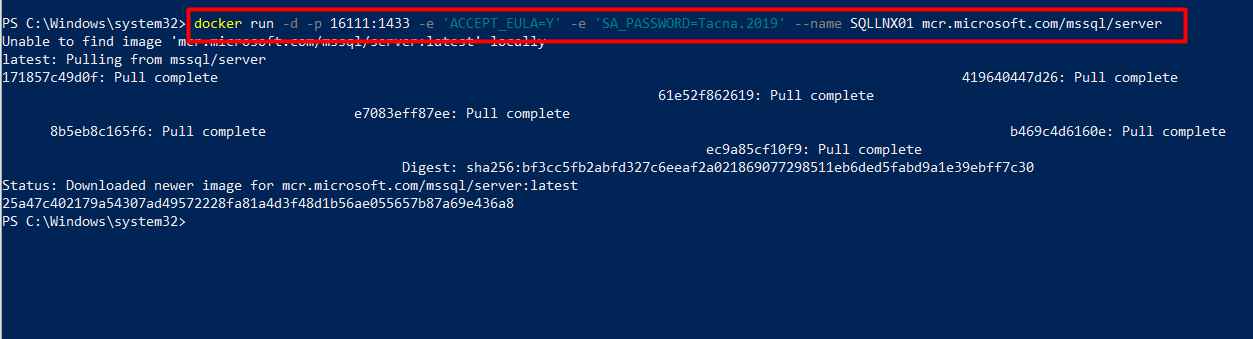
\includegraphics[width=15cm]{./images/1} 
	\end{center}

\textbf{2. Nos conectamos con usuario: sa y clave: Tacna.2020 
}

    \begin{center}
		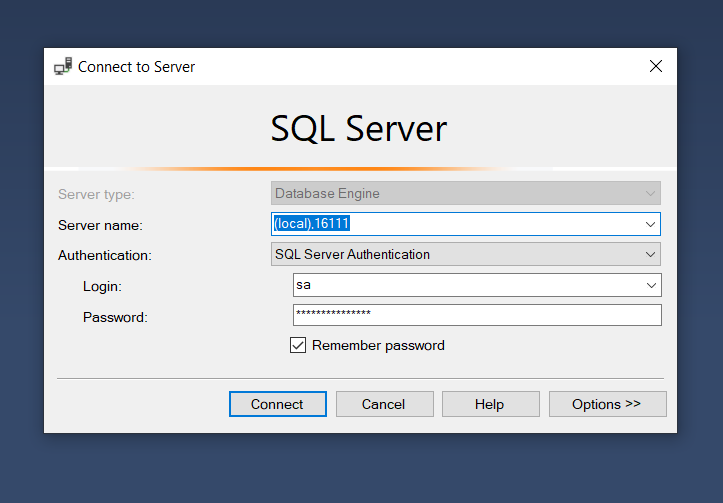
\includegraphics[width=15cm]{./images/2} 
	\end{center}
  \newpage
\textbf{3. Restauramos la base de datos}

    \begin{center}
		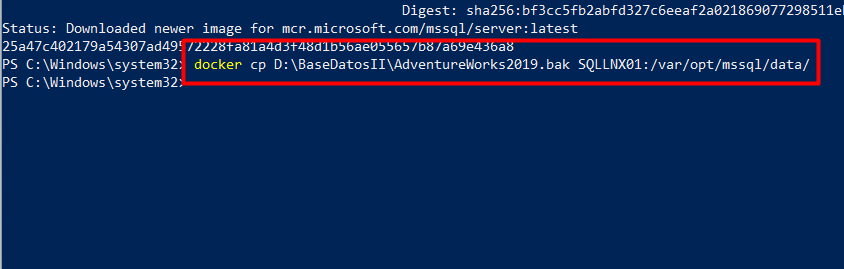
\includegraphics[width=15cm]{./images/3} 
	\end{center}
	
    \begin{center}
		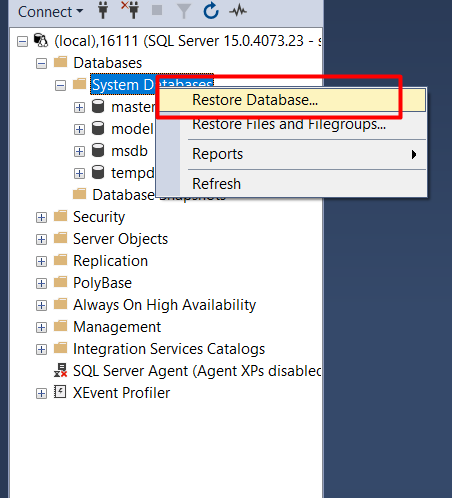
\includegraphics[width=15cm]{./images/4} 
	\end{center}
	
    \begin{center}
		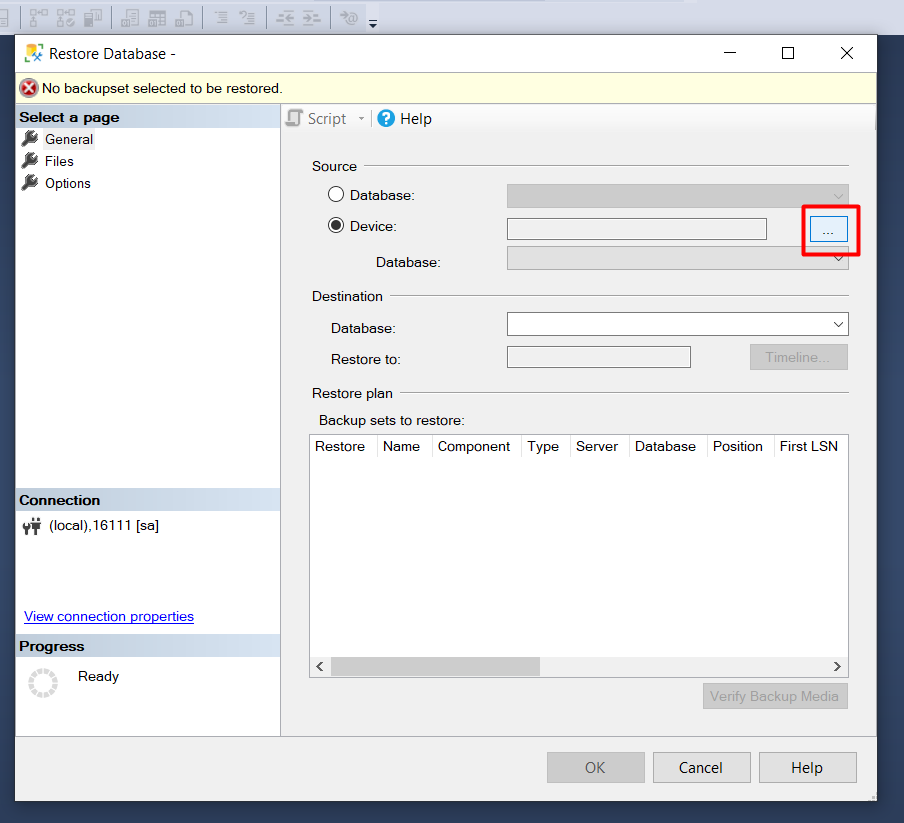
\includegraphics[width=15cm]{./images/5} 
	\end{center}
	
    \begin{center}
		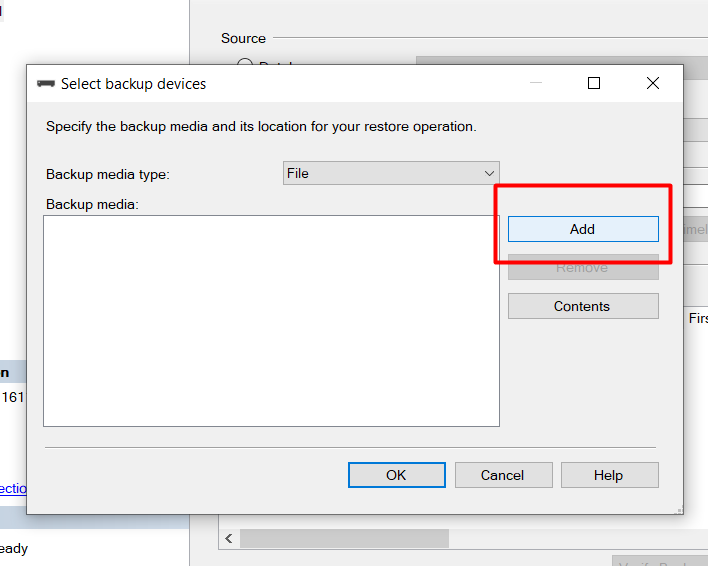
\includegraphics[width=15cm]{./images/6} 
	\end{center}

    \begin{center}
		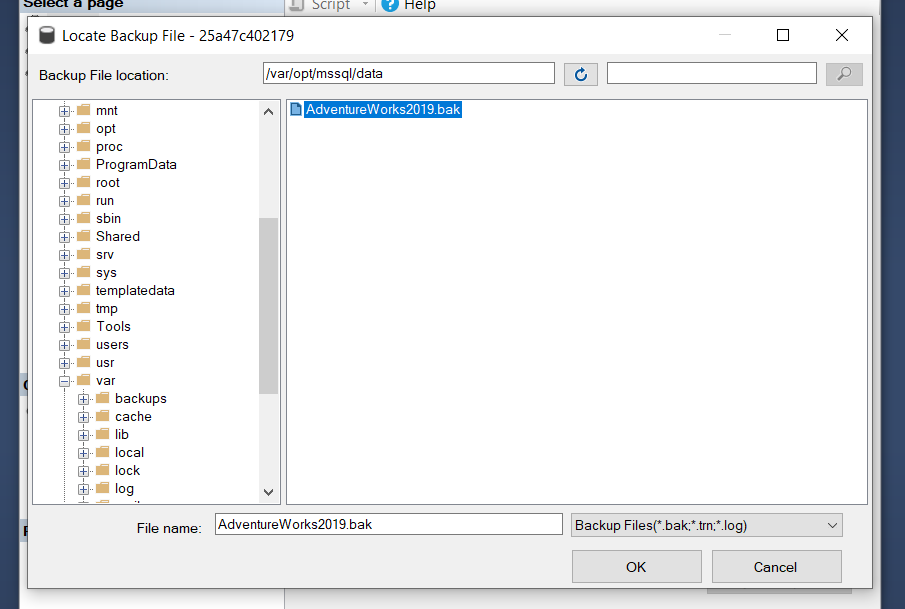
\includegraphics[width=15cm]{./images/7} 
	\end{center}
\textbf{4. Crear una auditoría del servidor con las siguientes propiedades.}

    \begin{center}
		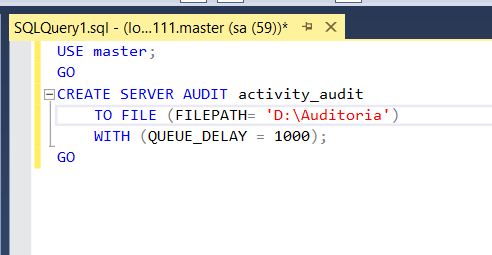
\includegraphics[width=15cm]{./images/8} 
	\end{center}
	

\textbf{5.  Activar la auditoria del servidor creada.}

   \begin{center}
		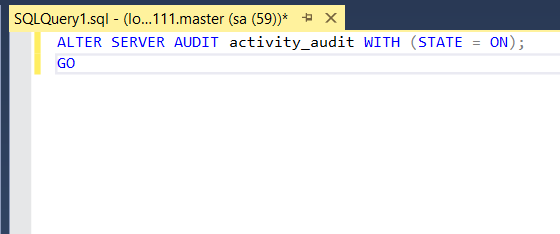
\includegraphics[width=15cm]{./images/9} 
	\end{center}

\textbf{6. Crear una especificación de auditoría del servidor con las siguientes propiedades.}

    \begin{center}
		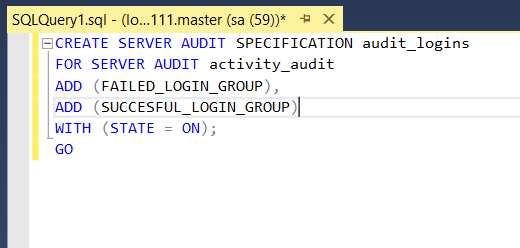
\includegraphics[width=15cm]{./images/10} 
	\end{center}
	
\newpage
\textbf{7.  Activar la especificación de auditoria del servidor creada.}

    \begin{center}
		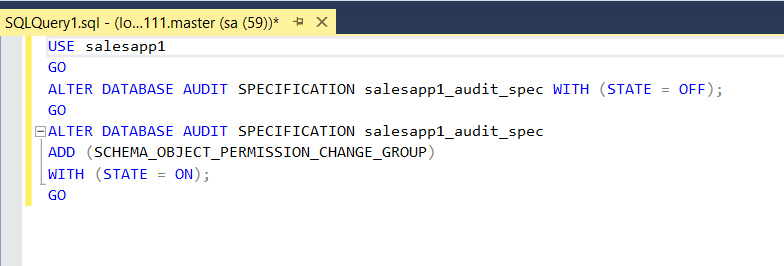
\includegraphics[width=15cm]{./images/11} 
	\end{center}
\textbf{8. Crear una especificación de auditoría de base de datos en la base de datos salesapp1 con las siguientes propiedades:}

    \begin{center}
		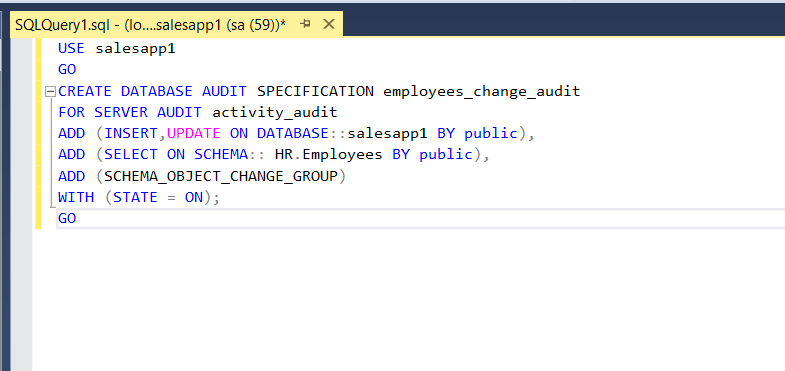
\includegraphics[width=15cm]{./images/12} 
	\end{center}

\newpage
\textbf{9. Activar la especificación de auditoría de base de datos creada.}

    \begin{center}
		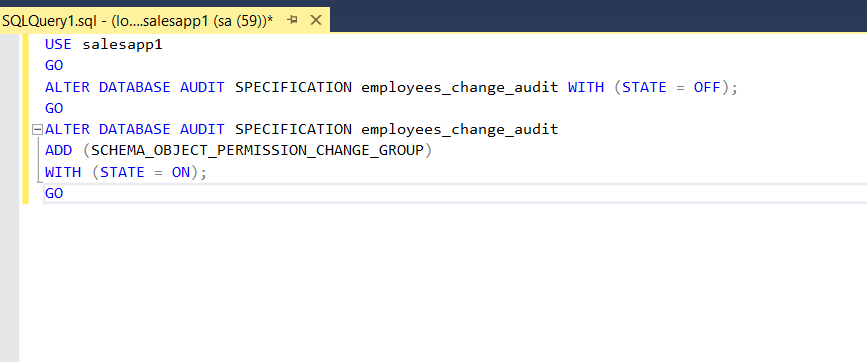
\includegraphics[width=15cm]{./images/13} 
	\end{center}

\textbf{10. Ejecutar el siguiente código}

    \begin{center}
		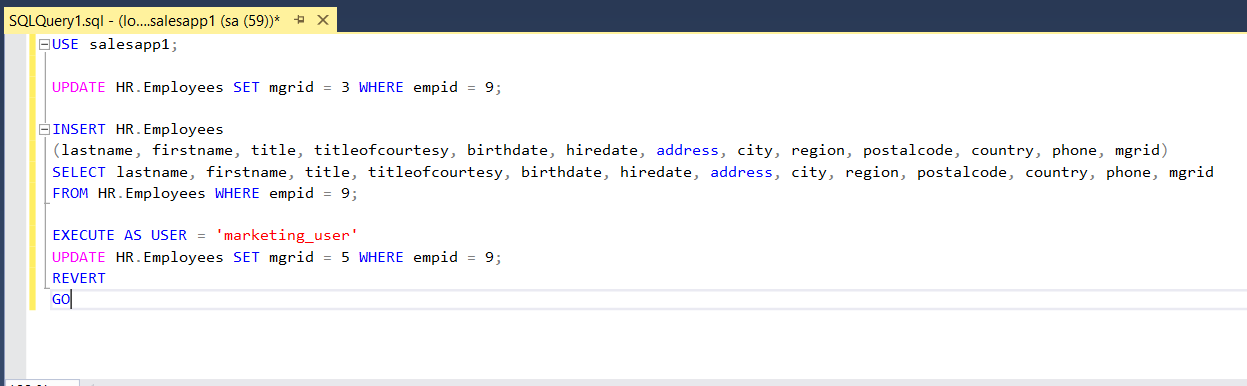
\includegraphics[width=15cm]{./images/14} 
	\end{center}


\newpage
\textbf{11.  Escribir una consulta utilizando la función de sistema sys.fn_get_audit_file para devolver todos los datos de auditoría desde los archivos en D:\Auditoria. Filtrar los datos para que solo la actividad relacionada a la sesión actual sea visualizada.}

    \begin{center}
		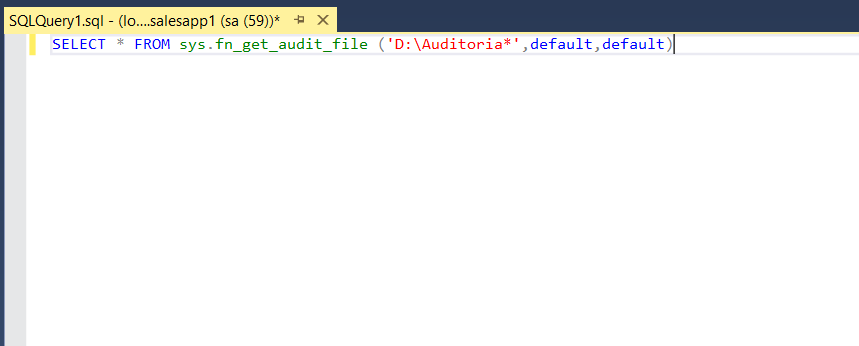
\includegraphics[width=15cm]{./images/15} 
	\end{center}

\textbf{12.  Desahbilitar la auditoría de servidor activity_audit.}

    \begin{center}
		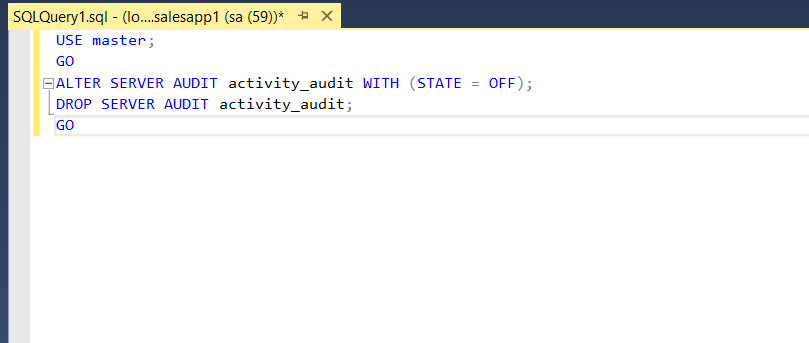
\includegraphics[width=15cm]{./images/16} 
	\end{center}
   
\end{document}
